\chapter{Grundlagen}

In diesem Kapitel sollen alle verwendeten Komponenten und Technologien kurz erklärt werden.
\section{ZigBee}

Die ZigBee Alliance wurde durch die Hersteller \todo{Zigbee Gründer} gegründet, um einen einheitlichen Übertragungstandard
voranzubringen. ZigBee basiert zwar auf einem offenem IEEE Standard, bringt aber Lizenzpflichtige Komponenten mit.
Dies verhindert leider maßgeblich eine weitere Ausbreitung des Standards.

ZigBee ist ein Kommunikationsprotokoll, welches im Bereich Iot Anwendungen findet. Das Protokoll baut auf dem Standard
802.40 auf. Genutzt wird es, um IoT fähige Geräte in einem Haushalt, wie zum Beispiel Lampen, Schalter oder Thermostate
zur Kommunikation zu befähigen. Markantetes Merkmal am Protokoll ist, dass die Geräte keine direkte Funkverbindung
zu einem zentralen Controlle brauchen, sondern über andere ZigBee fähige Geräte ein Netzwerk aufbauen. Vorteil ist,
dass ein im Vergleich zur benötigten Sendeleistung sehr großer Radius und Anahl von Geräten abgedeckt werden kann.

ZigBee erweitert den IEEE Standard um \todo{Zigbee erweiterungen}


\section{Texas Instruments CC Chips}

Texas Instruments bietet ein großes Spektrum von Microcontrollern, die den Zigbee Standard beherschen. Die Chips 
lassen sich in SDK Kits erwerben um eigene Firmwares zu entwickeln. Ebenfalls lassen sich im Internet sehr günstige
USB-Donge erwerben, welche sich nach belieben Flashen lassen. Dies erspart eine sehr aufwendige PCB Entwicklung
oder das erwerben des kostenspieligen SDK Kits von Texas Instruments.

Die aktuelle Chipfamilie TexasInstruments CC26XX:

\begin{figure}[H]
  \centering
  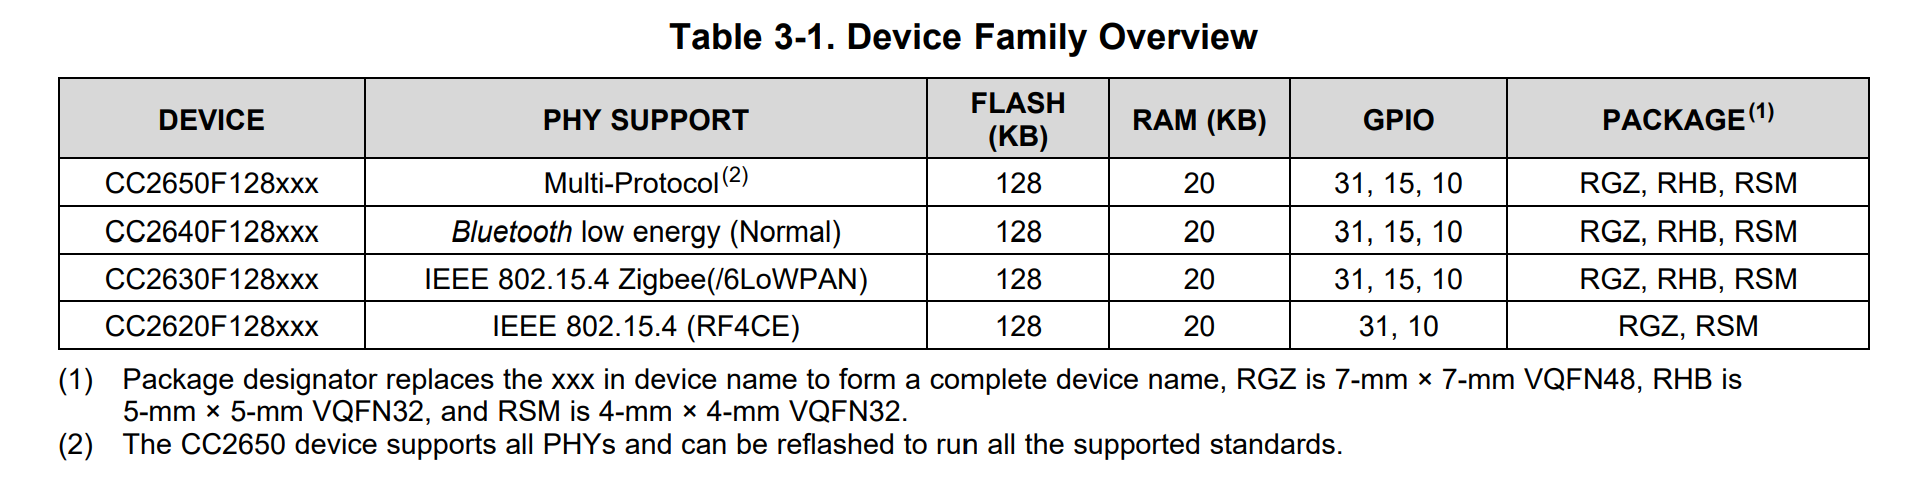
\includegraphics[width=1\textwidth]{media/table26xx.png}
  \caption{Test des Messagebrokers Mosquitto}
\end{figure}

Als Koordinator werden die Leistungsfähigeren Chips aus der 265X Reihe eingesetzt. ZigBee Geräte nutzen in manchen
Fällen Bluetooth LE zur Koppelung, daher ist die simultane Unterstüzung diesen Protokolls sinnvoll.

\begin{figure}[H]
  \centering
  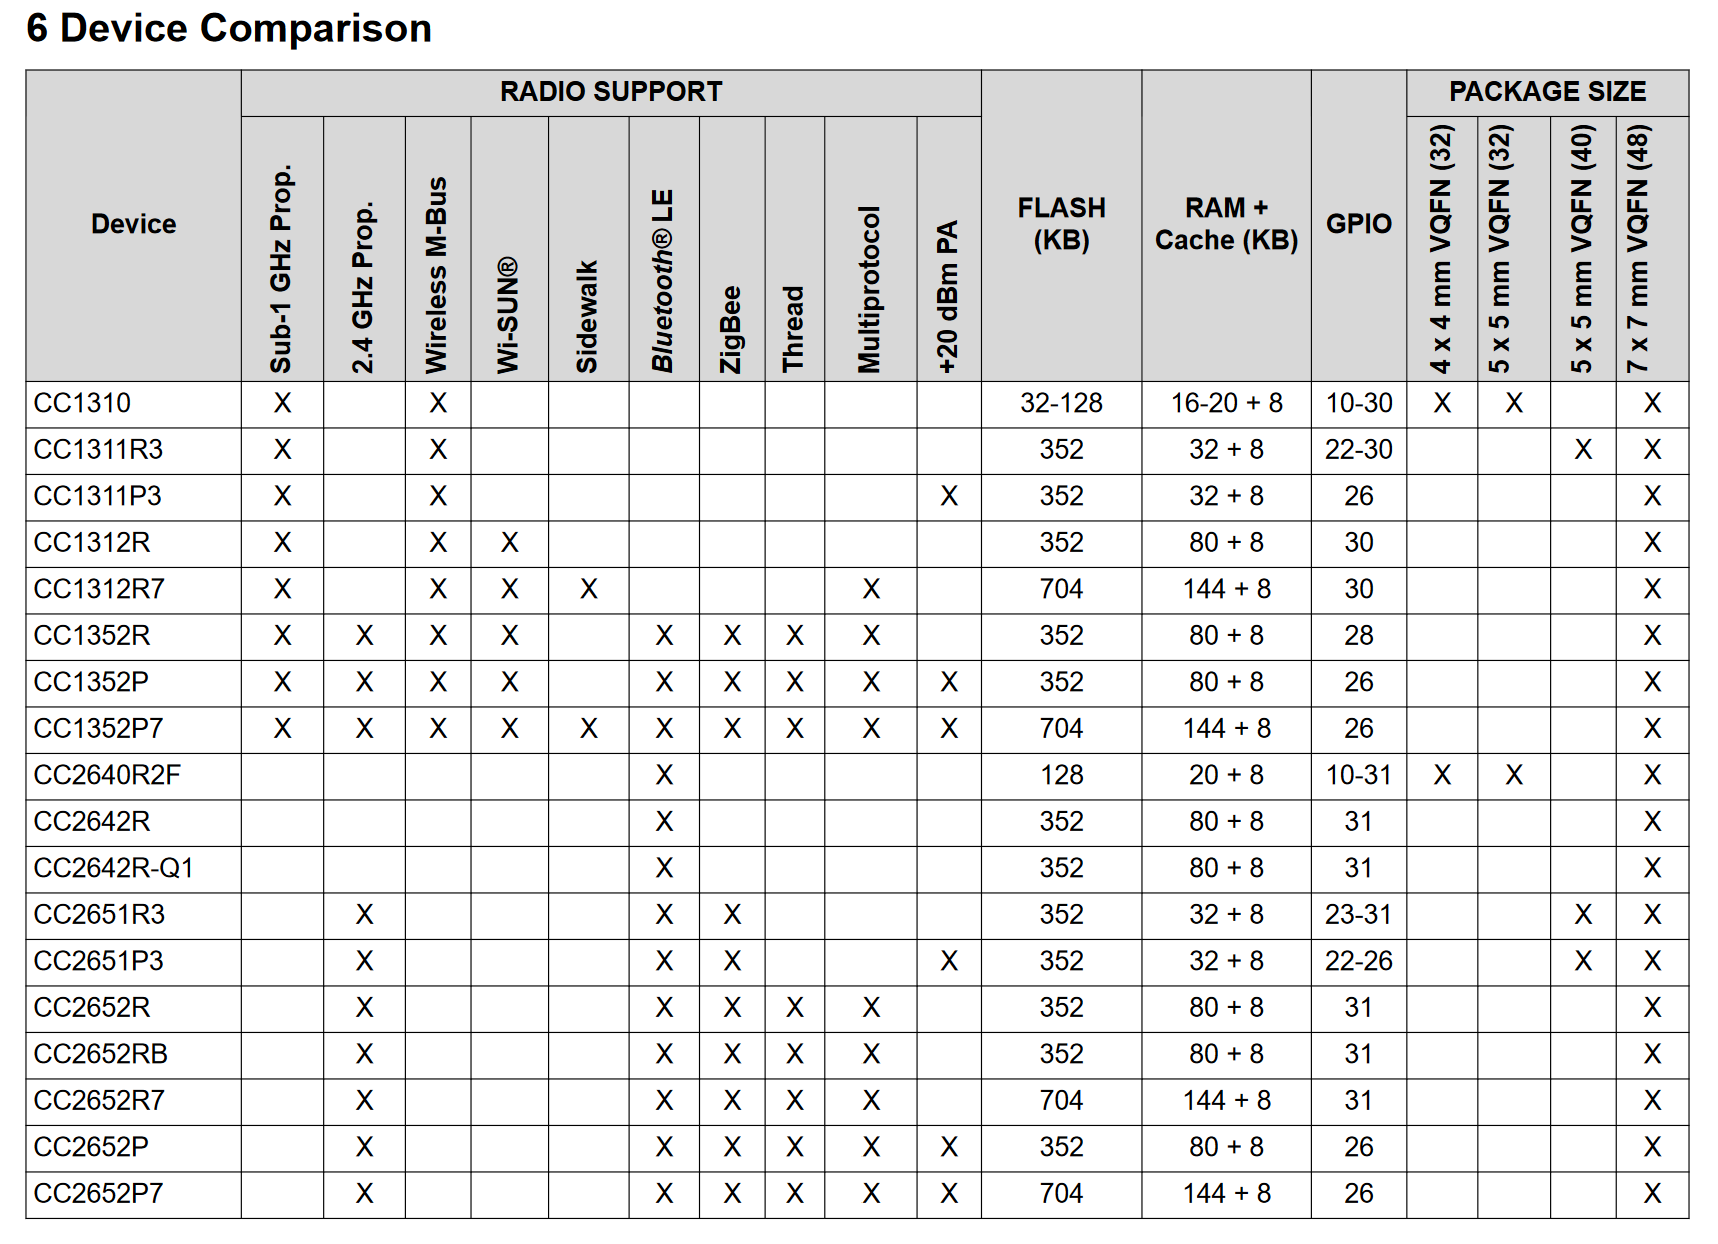
\includegraphics[width=1\textwidth]{media/table265x.png}
  \caption{Test des Messagebrokers Mosquitto}
\end{figure}

Hier in der Tabelle sind die unterstützten Protokolle der einzelnen Modelle sowie deren Leistungsfähigkeit aufgeführt.
Spannenderweise ist zu sehen, dass die Top Modelle schon den Standard Thread unterstützen, der vermutlich durch das
Projekt "Matter" erheblich an bedeutung gewinnt.

Texas Instruments bietet als Basis für ZigBee Eigententwicklungen eine Z-Stack Bibliothek. Diese stellt grundlegende 
Funktionen um das ZigBee Protokoll zu implementieren. Mit TexasInstruments Code Composer Studio steht eine IDE bereit,
um den Entwicklungsprozess zu unterstützen.

In dem OpenSource Projekt "zigbee2mqtt" werden ausschließlich Chips von Texas Instruments unterstützt. Es sei erwähnt, 
dass die meißten gängigen Anbieter von Microchips entsprechende Modelle im Angebot haben. 

\section{Versuchshardware}

\subsection{RaspberryPi}

Der RaspberryPi ist ein ARM basierter Computer im Mini-Format. Er dient in diesem Versuch als Server, der die Applikationen
hostet und gleichzeitig als Versuchs PC, von dem der Versuch aus ausgeführt wird. Die eingesetzten Dienste sind alle
als Webservice implementiert, und daher vollständig auf Kommandozeile parametrierbar, sowie mit WebGUI bedienbar.

Der RaspberryPi besitzt die Nutzer PC typtischen Schnittstellen wie Ethernet, HDMI, sowie USB. Als Hauptspeicher wird eine
SD-Karte eingestzt. Dies ist ein erheblicher Vorteil beim vorbereiten mehrerer RaspberryPis für den Versuch.

Auf dem RaspberryPi wird das Linux-basierte Betriebssystem RaspbyanOS eingesetzt. Durch die enorme Verbreitung ist
hier mit regelmäígen Updates in Zukunft zu rechnen.

\subsection{RaspberryPi Zigbee Hat}

Als Zigbee Koordinator kommt ein auf dem TI CC2652 basierendem RaspberryPi Hat zum Einsatz. Dieser wird mit einer Firmware aus dem zigbee2Mqtt Repository
geflasht. 

\subsection{CC2235 Sniffer Stick}

Mit diesem Stick wird die ZigBee Kommunikation zwischen dein einzelnen Devices sowie dem Koordinator mitgeschnitten auf einem bestimmten Kanal mitgeschnitten.

\subsection{Phillips Hue Komponenten}

Die Lampen werden in dem Versuch als Demonstrationsobjekte eingesetzt. Sie können Ein- und Ausgeschaltet werden, sowie gedimmt werden. Zusätzlich wird einer
Phillips Hie Fernbedienung verwendet, die zur Steuerung der Lampen dient.

\section{Eingesetzte Software}

\subsection{Raspbian OS}

RaspbianOS ist eine Linux Distribution, welche direkt vom Hersteller des RaspberryPis speziell auf die Bedürfnisse des Board angepasst werden. Es enthällt eine
Desktop Umgebung sowie die Grundlegend wichtigen Paketen. Es basiert auf Debian, damit sind auch die entsprechenden Paketquellen verfügbar.

\subsection{Docker}

Docker ist eine Container Umgebung, um Anwendungen containerisiert auf Linux-Servern laufen lassen zu können. Docker reduziert erheblich den Aufwand, 
Anwendungen auf mehreren Server auszurollen. Alle Abhängigkeiten sind im Container enthalten, sodass hier keine Komplikationen mit anderen Anwendungen
zu befürchten sind.

\subsection{zigbee2mqtt}

zigbee2mqtt ist ein offenes Softwareprojekt auf Zigbee, welches aus mehreren Komponenten besteht.

\subsubsection{TI CC Firmware}

Firmware für die Texas Instruments Chips, um diese als Koordinator einsetzen zu können. Die Firmware basiert auf dem Z-Stack von Texas Instruments.

\subsubsection{zigbee-herdman}

Dieses Modul verbindet sich direkt mit dem Zigbee Adapter, und steuert Ihn über die TI zStack monitoring and test API. \cite{zstack}

\subsubsection{zigbee-herdman-converters}

Dieser Konverter kann proprietäre Cluster die durch Geräte exposed werden umwandeln in standard Cluster. Mit diesem Converter lassen sich sämtliche Geräte
so adaptieren, dass sie nach Wunsch gesteuert und ausgelesen werden können.

\subsubsection{zigbee2mqtt}

Das Hauptmodul stellt die WebGui sowie eine Webanwendung mit einer SQLite Datenbank. Die Webanwendung und die Datenbank
verwalten den Zustand des Netzwerkes und die angebundenen Geräte. Die WebGUI dient zur Administration des Koordinators.

\todo{ Bild von zigbee2mqtt }

Die WebGUI enthällt eine große Anzahl von Funktionen, die weitaus tiefer reichen als für die Nutzung notwendig sind.
Prinzipiell sind die meißten ZigBee Geräte direkt Einsatzfähig, wenn ein Community Mitglied dieses bereits in der Anwendung
angelegt hat. Es ist auch möglich, eigene Beschreibungen für nich nicht unterstützte Geräte zu erstellen.


\subsection{Wireshark}

Wireshark ist eine quelloffene Anwendung um Datenstöme Mitzuschneiden und zu Untersuchen. Es kann durch Verwendung
von Packetsniffern wie nPcap verschiedenste Medien wie zum Beispiel Ethernet und USB mit entsprechenden Protokollen
verarbeiten.
